\documentclass[12pt,letterpaper]{exam}

\newcommand{\DocTitle}{Renew the DocTitle variable.}
\newcommand{\CourseNumber}{NE555}
\newcommand{\CourseName}{Nuclear Reactor Dynamics}
\newcommand{\DayTime}{TuTh 8:00-9:15}
\newcommand{\Room}{VV\&E B129}
\newcommand{\Term}{Spring 2011}
\newcommand{\Instructor}{Lewis John Lloyd}
\newcommand{\School}{University of Wisconsin - Madison}

\usepackage{listings}
\usepackage{mathtools}
\usepackage{xtab}
\usepackage{longtable}
\usepackage{array}
\usepackage{mathrsfs}
\usepackage{color}
\usepackage{multicol}
\usepackage{pdflscape}
\usepackage{pdfpages}
\usepackage{graphicx}
\usepackage{esint}
\usepackage{amsmath}
\usepackage{amssymb}
\usepackage{graphics}

\usepackage[
			pdfborder={0 0 0},
			urlcolor=cyan,
			pdftitle={\CourseNumber \DocTitle},
			pdfauthor={\Instructor}
			]{hyperref}
			
\usepackage[
			includeheadfoot,
			top=0.5in,
			bottom=0.5in,
			left=1.0in,
			right=1.0in
			]{geometry}
\setlength{\parindent}{0in}
\setlength{\parskip}{\baselineskip}

\lhead{\CourseNumber: \CourseName}
\chead{}
\rhead{\Term}
\lfoot{}
\cfoot{\thepage}
\rfoot{}
\coverlhead{\CourseNumber: \CourseName}
\coverchead{}
\coverrhead{\Term}
\coverlfoot{}
\covercfoot{\School}
\coverrfoot{}


\correctchoiceemphasis{\bfseries\color{red}}
\bracketedpoints
\pointsinmargin
%\addpoints
%\shadedsolutions

\lstset{ %
language=Matlab,                % the language of the code
basicstyle=\footnotesize,       % the size of the fonts that are used for the code
numbers=left,                   % where to put the line-numbers
numberstyle=\footnotesize,      % the size of the fonts that are used for the line-numbers
stepnumber=5,                   % the step between two line-numbers. If it's 1, each line 
                                % will be numbered
numbersep=5pt,                  % how far the line-numbers are from the code
backgroundcolor=\color{white},  % choose the background color. You must add \usepackage{color}
showspaces=false,               % show spaces adding particular underscores
showstringspaces=false,         % underline spaces within strings
showtabs=false,                 % show tabs within strings adding particular underscores
frame=single,                   % adds a frame around the code
tabsize=2,                      % sets default tabsize to 2 spaces
}

\renewcommand{\solutiontitle}{\noindent\textbf{Solution:}\par\noindent}

\newcommand{\mathsym}[1]{{}}
\newcommand{\unicode}{{}}
\newcommand{\tr}[1]{\tilde{#1}}
\newcommand{\LapTran}[1]{\mathscr{L}\left[#1\right]}
\newcommand{\InvLapTran}[1]{\mathscr{L}^{-1}\left[#1\right]}
\newcommand{\ParDer}[2]{\frac{\partial #1}{\partial #2}}
\newcommand{\Der}[2]{\frac{d\; #1}{d\;#2}}


\renewcommand{\DocTitle}{Problem Set 02}
\noprintanswers

%-------------------------------------------------------------------------------------
\begin{document}
%-------------------------------------------------------------------------------------
\begin{center}
\textbf{\DocTitle}
\end{center}
%-------------------------------------------------------------------------------------

\begin{questions}
%-------------------------------------------------------------------------------------
\question[15]{
O \& N: Chapter 3: Homework Problems: 1\\
Find $\bar{v}$ and the generation time $\Lambda$ for thermal neutrons.
Calculate $\bar{v}$ as the spectrum average for a normalized Maxwell spectrum:
$$\phi(E)dE = \frac{E}{kT}e^{-\frac{E}{kT}}\frac{dE}{kT}$$
Use T = 900 K and $\nu\Sigma_f$ = 0.3/cm.
\fullwidth{\begin{solution}
We trying to find $\displaystyle \langle v \rangle$.
Since the kinetic energy of a particle is $\displaystyle E\,=\,\frac{m_n v^2}{2}$, we get $\displaystyle v = \sqrt{\frac{2}{m}}\sqrt{E}$.
So, to get $\displaystyle \langle v \rangle$ we need $\displaystyle \sqrt{\frac{2}{m}}\langle \sqrt{E}\rangle$.
We are given $\displaystyle P(E)\,dE = \frac{E}{kT}e^{-\frac{E}{kT}}\frac{dE}{kT}$, so $\displaystyle \langle \sqrt{E} \rangle = \int\limits_{0}^{\infty}\,\sqrt{E}\,P(E)\,dE$. 
This yields an equation for the expected velocity:
$$\langle v \rangle = \sqrt{\frac{2}{m}} \int\limits_{0}^{\infty}\,\frac{E^{\frac{3}{2}}}{kT}e^{-\frac{E}{kT}}\frac{dE}{kT}$$
Numerically, we get $\displaystyle \langle v \rangle = 5120 \, [\frac{m}{s}]$, which when used with the given value of $\nu\Sigma_f$ = 0.3/cm, gives $\Lambda$ = 6.51 [$\mu$s].
\end{solution}}}
\ifprintanswers
\pagebreak
\fi
%-------------------------------------------------------------------------------------
\question{
O \& N: Chapter 3: Homework Problems: 2\\
Find $\bar{v}$ and $\displaystyle\overline{\left(\frac{1}{v}\right)}$ for a two group representation of a thermal reactor spectrum, composed for simplicity of a Maxwellian and a $\frac{1}{E}$ spectrum:

\begin{minipage}{0.4\linewidth}
\begin{eqnarray*}
\phi_{1}(E) & = & \frac{a}{E} \\
\phi_{2}(E) & = & \frac{b\,E}{(k\,T)^2}\;e^{-\frac{E}{k\,T}}
\end{eqnarray*}
\end{minipage}
\begin{minipage}{0.4\linewidth}
\begin{eqnarray*}
&,&for\; 0.2\; \textbf{eV}\; \leq E \leq 2\; \textbf{MeV} \\
&,&for\; 0\; \leq E \leq \infty
\end{eqnarray*}
\end{minipage}

\begin{parts}
% Part 01--------------------------------------------------------------------------------
\part[5]{Find \textit{a} and \textit{b} such that the two components of the normalized $\phi(E)$ provide equal contributions to the energy integral.}
\fullwidth{\begin{solution}
\begin{minipage}{0.4\linewidth}
\begin{eqnarray*}
1 & = & \int\limits_{0.2\,eV}^{2.0\,MeV}\,\phi_1\,dE + \int\limits_{0}^{\infty}\,\phi_2\,dE\\
1 & = & a\,7\,ln|10| + b\\
1 & = & a\,14\,ln|10|\\
a & = & \frac{1}{14\,ln|10|}\\
a & = & 0.031
\end{eqnarray*}
\end{minipage}
\begin{minipage}{0.4\linewidth}
\begin{eqnarray*}
\int\limits_{0}^{\infty}\,\phi_2\,dE & = & \int\limits_{0.2\,eV}^{2.0\,MeV}\,\phi_1\,dE \\
b & = & a\,7\,ln|10|\\
b & = & \frac{7\,ln|10|}{14\,ln|10|}\\
b & = & 0.5
\end{eqnarray*}
\end{minipage}
\end{solution}}

% Part 02--------------------------------------------------------------------------------
\part[4]{Find the average velocities for both groups ($\bar{v}_1$ and $\bar{v}_2$). If necessary, leave as a function of temperature, T, in [K].}
\fullwidth{\begin{solution}
\begin{eqnarray*}
\langle v_1 \rangle & = & \sqrt{\frac{2}{m_n}}\frac{\int\limits_{0.2\,eV}^{2.0\,MeV}\,\sqrt{E}\phi_1(E)\,dE}{\int\limits_{0.2\,eV}^{2.0\,MeV}\,\phi_1(E)\,dE}\\
& = & 2.428\cdot 10^{6}\; [\frac{m}{s}]
\end{eqnarray*}
\begin{eqnarray*}
\langle v_2 \rangle(T) & = & \sqrt{\frac{2}{m_n}}\frac{\int\limits_{0}^{\infty}\,\sqrt{E}\phi_2(E)\,dE}{\int\limits_{0}^{\infty}\,\phi_2(E)\,dE}\\
& = & 170.685\; \sqrt{T}\; [\frac{m}{s}]
\end{eqnarray*}
\end{solution}}

% Part 03--------------------------------------------------------------------------------
\part[4]{Express the two group definitions of $\bar{v}$ and $\displaystyle\overline{\left(\frac{1}{v}\right)}$ as functions of temperature, T, in [K].}
\fullwidth{\begin{solution}
\begin{eqnarray*}
\langle v \rangle(T) & = & \sqrt{\frac{2}{m_n}}\frac{\int\limits_{0.2\,eV}^{2.0\,MeV}\,\sqrt{E}\phi_1(E)\,dE+\int\limits_{0}^{\infty}\,\sqrt{E}\phi_2(E)\,dE}{\int\limits_{0.2\,eV}^{2.0\,MeV}\,\phi_1(E)\,dE+\int\limits_{0}^{\infty}\,\phi_2(E)\,dE}\\
& = & 1.2\cdot 10^{6}+85.3\; \sqrt{T}\; [\frac{m}{s}]
\end{eqnarray*}
\begin{eqnarray*}
\langle \frac{1}{v} \rangle(T) & = & \sqrt{\frac{m_n}{2}}\frac{\int\limits_{0.2\,eV}^{2.0\,MeV}\,\frac{1}{\sqrt{E}}\phi_1(E)\,dE+\int\limits_{0}^{\infty}\,\frac{1}{\sqrt{E}}\phi_2(E)\,dE}{\int\limits_{0.2\,eV}^{2.0\,MeV}\,\phi_1(E)\,dE+\int\limits_{0}^{\infty}\,\phi_2(E)\,dE}\\
& = & 9.983\cdot 10^{-6}+\frac{0.00345109}{\sqrt{T}}\; [\frac{m}{s}]
\end{eqnarray*}
\end{solution}}

% Part 04--------------------------------------------------------------------------------
\part[2]{Find the corresponding numerical values for T = 900 [K].}
\fullwidth{\begin{solution}
\begin{eqnarray*}
\langle v \rangle(900) & = & 1.22\cdot 10^{6}\; [\frac{m}{s}]\\
\langle \frac{1}{v} \rangle(900) & = & 1.24\cdot 10^{-4}\; [\frac{s}{m}]
\end{eqnarray*}
\end{solution}}
\end{parts}}
\ifprintanswers
\pagebreak
\fi
%-------------------------------------------------------------------------------------
\question[5]{
O \& N: Chapter 3: Review Questions: 6\\
Give two equivalent differential equations for the power of a nuclear reactor.
Have one equation use $k$ \& \textit{l} and the other use $\rho$ \& $\Lambda$. 
Treat \textbf{all} neutrons as prompt and neglect external sources.
\fullwidth{\begin{solution}
\begin{eqnarray*}
\frac{\partial P}{\partial t} & = & \frac{\rho}{\Lambda}P\\
\frac{\partial P}{\partial t} & = & \frac{k-1}{\textit{l}}P
\end{eqnarray*}
\end{solution}}}
\ifprintanswers
\pagebreak
\fi
%-------------------------------------------------------------------------------------
\question{
Using the answer from Question 3 that contains $\rho$ \& $\Lambda$, account for the presence of a constant external source of neutrons in the reactor by introducing $S_o$, expressed in [J], into the differential equation.
\begin{parts}
%-------------------------------------------------------
\part[1]{What is the differential equation describing this new system? Be sure to provide the initial condition.}
\fullwidth{\begin{solution}
$$\displaystyle \frac{\partial P}{\partial t} = \frac{\rho}{\Lambda}P+S_o$$
\end{solution}}

%-------------------------------------------------------
\part[5]{Solve the differential equation for a constant $\rho$, such that $k \neq 1$.}
\fullwidth{\begin{solution}
\begin{eqnarray*}
\ParDer{P}{t} & = & \frac{\rho}{\Lambda}P + S_o\\
\ParDer{P}{t}-\frac{\rho}{\Lambda}P & = & S_o\\
\ParDer{P}{t}e^{-\frac{\rho}{\Lambda}t}-\frac{\rho}{\Lambda}e^{-\frac{\rho}{\Lambda}t}P & = & S_o\,e^{-\frac{\rho}{\Lambda}t}\\
\ParDer{\left(P\;e^{-\frac{\rho}{\Lambda}t}\right)}{t} & = & S_o\,e^{-\frac{\rho}{\Lambda}t}\\
\int\limits_{0}^{t} \ParDer{\left(P(t')\;e^{-\frac{\rho}{\Lambda}t'}\right)}{t'} dt' & = & \int\limits_{0}^{t}\;S_o\,e^{-\frac{\rho}{\Lambda}t'}dt'\\
\int\limits_{P(0)}^{P(t)e^{-\frac{\rho}{\Lambda}t}}\;df & = & \left[-\frac{S_o\Lambda}{\rho} e^{-\frac{\rho}{\Lambda}t}\right]_{0}^{t}\\
P(t)e^{-\frac{\rho}{\Lambda}t}-P(0) & = & -\frac{S_o\Lambda}{\rho} e^{-\frac{\rho}{\Lambda}t}+\frac{S_o\Lambda}{\rho}\\
P(t) & = & P(0)e^{\frac{\rho}{\Lambda}t}+\frac{S_o\Lambda}{\rho}\left(e^{\frac{\rho}{\Lambda}t}-1\right)
\end{eqnarray*}
\end{solution}}

%-------------------------------------------------------
\part[5]{Solve the differential equation for k = 1.}
\fullwidth{\begin{solution}
\begin{eqnarray*}
\ParDer{P}{t} & = & \frac{\rho}{\Lambda}P + S_o\\
\ParDer{P}{t} & = & S_o\\
\int\limits_{0}^{t} \ParDer{P(t')}{t'} dt' & = & S_o\int\limits_{0}^{t}\;dt'\\
\int\limits_{P(0)}^{P(t)}\;df & = & S_o \left[t'\,\right]_{0}^{t}\\
P(t)-P(0) & = & S_o\,t\\
P(t) & = & P(0)+S_o\,t\\
\end{eqnarray*}
\end{solution}}

%-------------------------------------------------------
\part[2]{What is the value of $k$ that renders a steady state solution for a source $S_o$?}
\fullwidth{\begin{solution}
\begin{eqnarray*}
\ParDer{P}{t} & = & \frac{\rho}{\Lambda}P + S_o\\
0 & = &\frac{k-1}{\textit{l}}P + S_o\\
\frac{k-1}{\textit{l}}P_o & = & -S_o\\
k-1 & = &  -\frac{S_o \textit{l}}{P_o}\\
k & = & 1 - \frac{S_o \textit{l}}{P_o}
\end{eqnarray*}
\end{solution}}

%-------------------------------------------------------
\part[1]{What is the steady state multiplication factor, M, for the reactor in terms of $k$?\\
\textbf{Note}: M = $\displaystyle\frac{P_o}{S_o}$}
\fullwidth{\begin{solution}
\begin{eqnarray*}
\ParDer{P}{t} & = & \frac{\rho}{\Lambda}P + S_o\\
0 & = &\frac{\rho}{\Lambda}P_o + S_o\\
\frac{P_o}{S_o} & = & -\frac{\Lambda}{\rho}\\
M & = & \frac{\textit{l}}{1-k}
\end{eqnarray*}
\end{solution}}

%-------------------------------------------------------
\part[1]{Plot $\displaystyle \frac{M}{\textit{l}}$ vs. k.}
\fullwidth{\begin{solution}
See next page for graph.
\end{solution}}
\end{parts}}
%-------------------------------------------------------------------------------------
\end{questions}
\ifprintanswers
\begin{landscape}
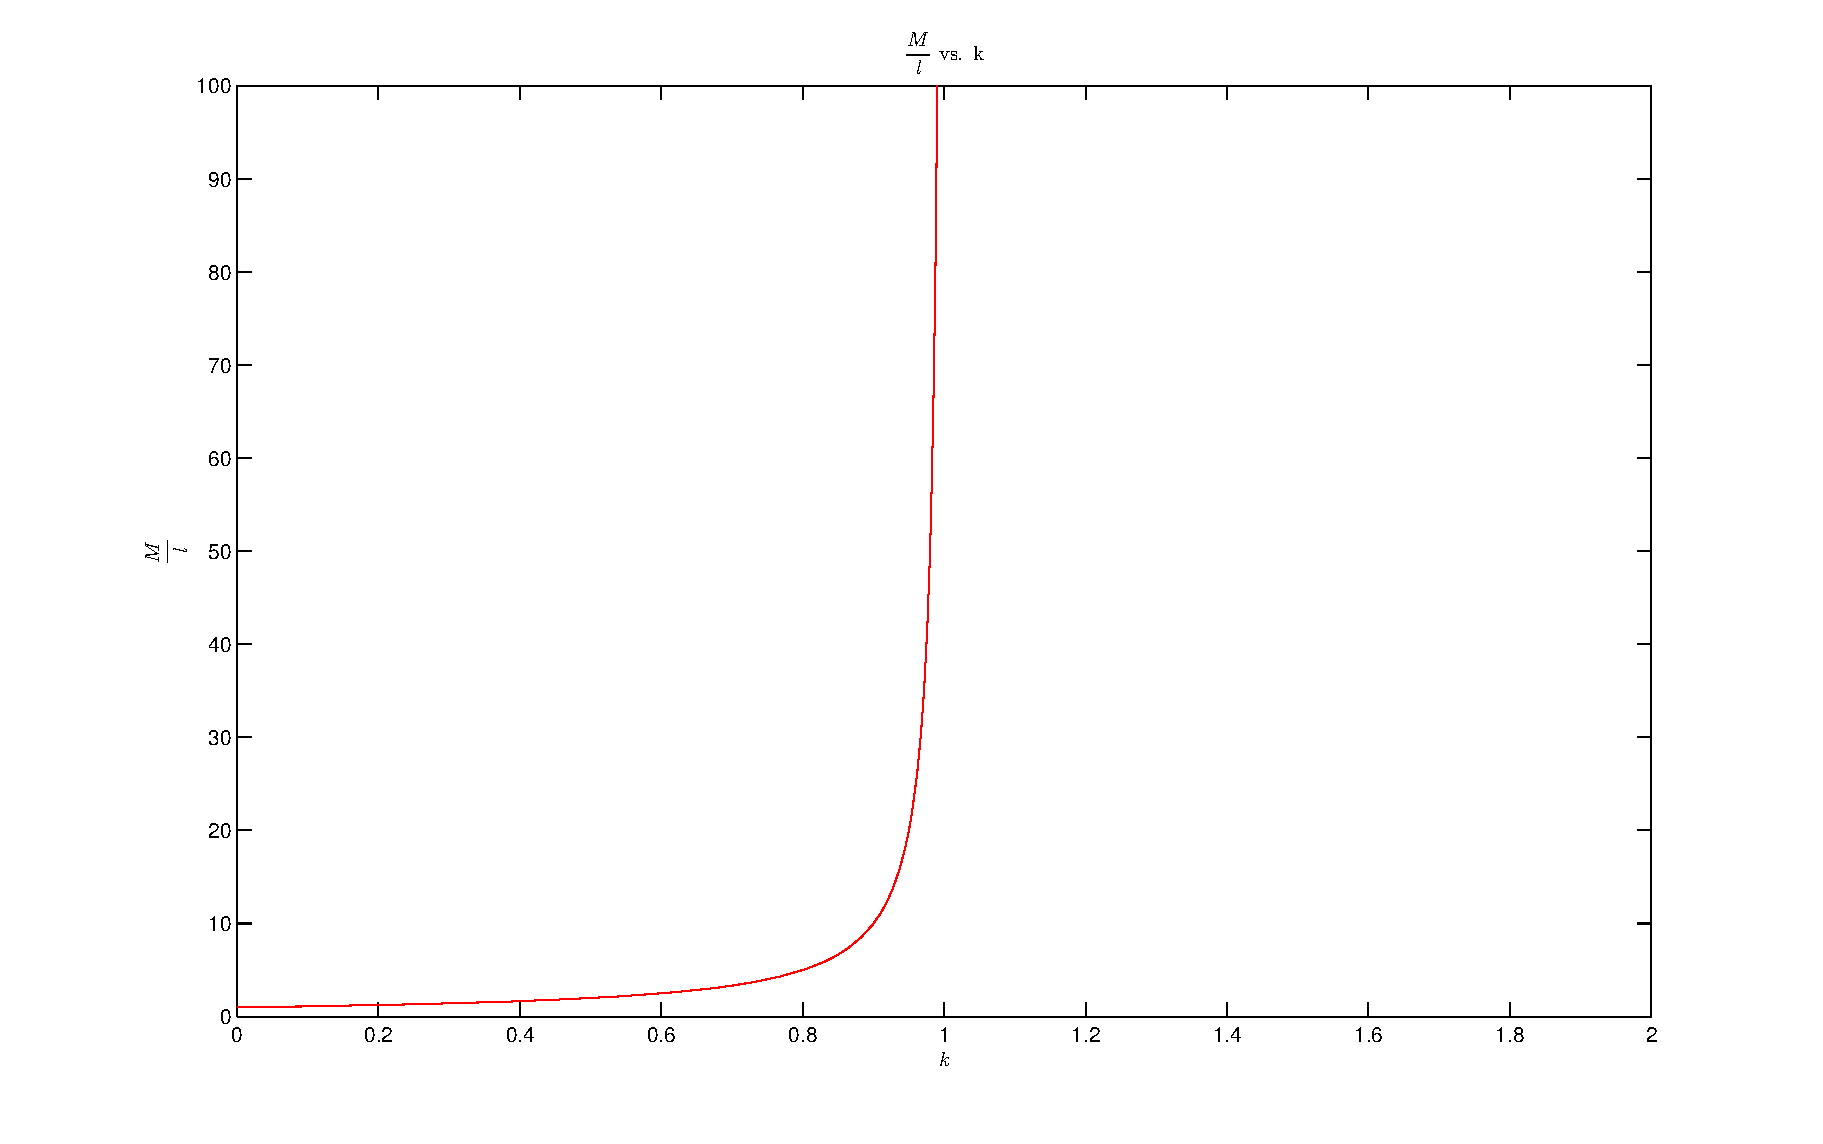
\includepdf[landscape=true]{PS02Q04pic.pdf}
\end{landscape}
\fi


\end{document}